%%%%%%%%%%%%%%%%%%%%%%%%%%%%%%%%%%%%%%%%%
% Short Sectioned Assignment LaTeX Template Version 1.0 (5/5/12)
% This template has been downloaded from: http://www.LaTeXTemplates.com
% Original author:  Frits Wenneker (http://www.howtotex.com)
% License: CC BY-NC-SA 3.0 (http://creativecommons.org/licenses/by-nc-sa/3.0/)
%%%%%%%%%%%%%%%%%%%%%%%%%%%%%%%%%%%%%%%%%

%----------------------------------------------------------------------------------------
%	PACKAGES AND OTHER DOCUMENT CONFIGURATIONS
%----------------------------------------------------------------------------------------

\documentclass[paper=a4, fontsize=11pt]{scrartcl} % A4 paper and 11pt font size

% ---- Entrada y salida de texto -----

\usepackage{hyperref}
\usepackage{varioref}
\usepackage[T1]{fontenc} % Use 8-bit encoding that has 256 glyphs
\usepackage[utf8]{inputenc}
%\usepackage{fourier} % Use the Adobe Utopia font for the document - comment this line to return to the LaTeX default

% ---- Idioma --------

\usepackage[spanish, es-tabla]{babel} % Selecciona el español para palabras introducidas automáticamente, p.ej. "septiembre" en la fecha y especifica que se use la palabra Tabla en vez de Cuadro

% ---- Otros paquetes ----

\usepackage{amsmath,amsfonts,amsthm} % Math packages
%\usepackage{graphics,graphicx, floatrow} %para incluir imágenes y notas en las imágenes
\usepackage{graphics,graphicx, float} %para incluir imágenes y colocarlas

% Para hacer tablas comlejas
%\usepackage{multirow}
%\usepackage{threeparttable}

%\usepackage{sectsty} % Allows customizing section commands
%\allsectionsfont{\centering \normalfont\scshape} % Make all sections centered, the default font and small caps

\usepackage{fancyhdr} % Custom headers and footers
\pagestyle{fancyplain} % Makes all pages in the document conform to the custom headers and footers
\fancyhead{} % No page header - if you want one, create it in the same way as the footers below
\fancyfoot[L]{} % Empty left footer
\fancyfoot[C]{} % Empty center footer
\fancyfoot[R]{\thepage} % Page numbering for right footer
\renewcommand{\headrulewidth}{0pt} % Remove header underlines
\renewcommand{\footrulewidth}{0pt} % Remove footer underlines
\setlength{\headheight}{13.6pt} % Customize the height of the header

\numberwithin{equation}{section} % Number equations within sections (i.e. 1.1, 1.2, 2.1, 2.2 instead of 1, 2, 3, 4)
\numberwithin{figure}{section} % Number figures within sections (i.e. 1.1, 1.2, 2.1, 2.2 instead of 1, 2, 3, 4)
\numberwithin{table}{section} % Number tables within sections (i.e. 1.1, 1.2, 2.1, 2.2 instead of 1, 2, 3, 4)

\setlength\parindent{0pt} % Removes all indentation from paragraphs - comment this line for an assignment with lots of text

\newcommand{\horrule}[1]{\rule{\linewidth}{#1}} % Create horizontal rule command with 1 argument of height


 \usepackage{algpseudocode}
%----------------------------------------------------------------------------------------
%	TÍTULO Y DATOS DEL ALUMNO
%----------------------------------------------------------------------------------------

\title{	
\normalfont \normalsize 
\textsc{{\bf Técnicas de los Sistemas Inteligentes (2015-2016)} \\ Grado en Ingeniería Informática \\ Universidad de Granada} \\ [25pt] % Your university, school and/or department name(s)
\horrule{0.5pt} \\[0.4cm] % Thin top horizontal rule
\huge Práctica 3: Primera Parte \\ % The assignment title
\horrule{2pt} \\[0.5cm] % Thick bottom horizontal rule
}

\author{Francisco Carrillo Pérez} % Nombre y apellidos

\date{\normalsize\today} % Incluye la fecha actual

%----------------------------------------------------------------------------------------
% DOCUMENTO
%----------------------------------------------------------------------------------------

\begin{document}

\maketitle % Muestra el Título

\newpage %inserta un salto de página

\tableofcontents % para generar el índice de contenidos

\listoffigures

\newpage

\section*{Introducción}
En el siguiente documento se va a proceder a la explicación a las decisiones de diseño que se han tomado a la hora de realizar 5 ejercicios de los 6 propuestos, además de mostrar los distintos planes que se han conseguido para cada dominio y problema.

\section{Ejercicio 1}
\subsection{Apartado a}
Para la representación en el dominio de los objetos en el mundo se ha optado por tener 4 tipos:
\begin{itemize}
	\item \textbf{robot}: Para representar al robot.
	\item \textbf{zona}: Para representar las distintas zonas dentro del mundo.
	\item \textbf{objeto}: Para representar los distintos objetos que hay en el mundo.
	\item \textbf{personaje}: Para representar a los distintos personajes que hay en el mundo.
\end{itemize}
Podemos observarlo de la siguiente forma en el archivo del domimio:
\begin{verbatim}
 (:types robot zona objeto personaje)
\end{verbatim}
\subsection{Apartado b}
Los predicados que se han descrito son los siguientes:
\begin{itemize}
	\item \textbf{(at ?x - robot ?y - zona)}: Para representar en que zona se encuentra el robot.
	\item \textbf{(at1 ?x - objeto ?y - zona)}: Para representar en que zona se encuentra un objeto.
	\item \textbf{(at2 ?x - personaje ?y - zona)}: Para representar en que zona se encuentra un personaje.
	\item \textbf{(conectada ?x - zona ?y - zona)}: Para representar que dos zonas se encuentran conectadas.
	\item \textbf{(cogido ?x - objeto)}: Para representar que el robot tiene cogido un determinado objeto.
	\item \textbf{(tiene ?x - objeto ?y - personaje)}: Para representar que un determinado personaje tiene un determinado objeto.
	\item \textbf{(manovacia)}: Para representar que el robot no tiene ningún objeto cogido.
\end{itemize}
Podemos observarlo de la siguiente forma en el archivo del domimio:
\begin{verbatim}
;Declaracion de los predicados del mundo de Belkan
(:predicates   
    (at ?x - robot ?y - zona)
    (at1 ?x - objeto ?y - zona)
    (at2 ?x - personaje ?y - zona)
    (conectada ?x - zona ?y - zona)
    (cogido ?x - objeto)
    (tiene ?x - objeto ?y - personaje)
    (manovacia)
)
\end{verbatim}
\subsection{Apartado c}
Las acciones se han representado de la siguiente forma:\\
\textbf{Ir de una zona a otra}\\
\begin{verbatim}
;Acción de movimiento del robot
(:action mover-robot
    :parameters (?r - robot ?z1 - zona ?z2 - zona)
    :precondition (and (not (at ?r ?z2))(at ?r ?z1)(conectada ?z1 ?z2))
    :effect (and (not (at ?r ?z1))(at ?r ?z2))
)
\end{verbatim}
Así tenemos:
\begin{itemize}
	\item \textbf{Parámetros}: El robot, la zona donde estamos y la zona a donde deseamos desplazarnos.
	\item \textbf{Precondiciones}: Que el robot no se encuentre en la zona a donde deseamos desplazarnos, que el robot se encuentre en la primera zona, y que ambas zonas estén conectadas, para poder desplazarnos de una a otra.
	\item \textbf{Efecto}: Que el robot no se encuentre en la primera zona donde estaba, y que ahora se encuentre en la segunda zona.\\
\end{itemize}
\textbf{Coger un objeto}\\
\begin{verbatim}
;Acción de coger un objeto
(:action coger-objeto
    :parameters (?r - robot ?obj - objeto ?obj1 - objeto ?z - zona)
    :precondition (and (at ?r ?z) (at1 ?obj ?z)(manovacia))
    :effect (and (not (manovacia))(cogido ?obj))

)
\end{verbatim}
Así tenemos:
\begin{itemize}
	\item \textbf{Parámetros}: El robot, el objeto que queremos coger y la zona donde nos encontramos y se encuentra el objeto.
	\item \textbf{Precondiciones}: Que el robot y el objeto se encuentren en la misma zona, y que tengamos la mano vacía.
	\item \textbf{Efecto}: El robot deja de tener la mano vacía y pasa a tener cogido el objeto.\\
\end{itemize}
\textbf{Dejar un objeto}\\
\begin{verbatim}
;Acción de dejar un objeto
(:action dejar-objeto
    :parameters (?r - robot ?obj - objeto ?z - zona)
    :precondition (and (at ?r ?z)(cogido ?obj))
    :effect (and (not (cogido ?obj))(at1 ?obj ?z)(manovacia))
)
\end{verbatim}
Así tenemos:
\begin{itemize}
	\item \textbf{Parámetros}: El robot, el objeto que queremosdejar y la zona donde nos encontramos y queremos dejar el objeto.
	\item \textbf{Precondiciones}: Que el robot y el objeto se encuentren en la misma zona, y que tengamos el objeto cogido.
	\item \textbf{Efecto}: El robot pasa a tener la mano vacía, deja cogido el objeto y se inserta que el objeto se encuentre en esa zona.\\
\end{itemize}
\textbf{Entregar un objeto a un personaje}\\
\begin{verbatim}
;Entregar un objeto a un personaje
(:action entregar-objeto
    :parameters(?r - robot ?obj - objeto ?z - zona ?p - personaje)
    :precondition (and (not (tiene ?obj ?p))(at ?r ?z)(at2 ?p ?z)(cogido ?obj))
    :effect (and (not (cogido ?obj))(tiene ?obj ?p)(manovacia))
)
\end{verbatim}
Así tenemos:
\begin{itemize}
	\item \textbf{Parámetros}: El robot, el objeto que queremos entregar . la zona donde nos encontramos y el personaje al que queremos entregar el objeto.
	\item \textbf{Precondiciones}: Que el personaje no tenga objeto, que el robot y el personaje estén en la misma zona y que tenga cogido el objeto.
	\item \textbf{Efecto}: El robot ya no tiene cogido el objeto, el personaje tiene el objeto y tiene la mano vacía.\\
\end{itemize}
\subsection{Apartado d}
El archivo de problema es el siguiente:
\begin{verbatim}
(define (problem Problema1)

(:domain LosMundosDeBelkan)

(:OBJECTS Z1 Z2 Z3 Z4 Z5 Z6 Z7 Z8 Z9 Z10 Z11 Z12 Z13 Z14 Z15 Z16 
Z17 Z18 Z19 Z20 Z21 Z22 Z23 Z24 Z25 - zona ROBOT - robot 
OSCAR MANZANA ROSA ALGORITMO ORO - objeto PRINCESA PRINCIPE BRUJA
PROFESOR LEONARDO - personaje)

(:INIT  (CONECTADA Z1 Z2)
(CONECTADA Z2 Z1)
(CONECTADA Z1 Z6)
(CONECTADA Z6 Z1)
(CONECTADA Z2 Z3)
(CONECTADA Z3 Z2)
(CONECTADA Z2 Z7)
(CONECTADA Z7 Z2)
(CONECTADA Z3 Z4)
(CONECTADA Z4 Z3)
(CONECTADA Z3 Z8)
(CONECTADA Z8 Z3)
(CONECTADA Z4 Z5)
(CONECTADA Z5 Z4)
(CONECTADA Z4 Z9)
(CONECTADA Z9 Z4)
(CONECTADA Z5 Z10)
(CONECTADA Z10 Z5)
(CONECTADA Z6 Z7)
(CONECTADA Z7 Z6)
(CONECTADA Z6 Z11)
(CONECTADA Z11 Z6)
(CONECTADA Z7 Z8)
(CONECTADA Z8 Z7)
(CONECTADA Z7 Z12)
(CONECTADA Z12 Z7)
(CONECTADA Z8 Z9)
(CONECTADA Z9 Z8)
(CONECTADA Z8 Z13)
(CONECTADA Z13 Z8)
(CONECTADA Z9 Z10)
(CONECTADA Z10 Z9)
(CONECTADA Z9 Z14)
(CONECTADA Z14 Z9)
(CONECTADA Z10 Z15)
(CONECTADA Z15 Z10)
(CONECTADA Z11 Z12)
(CONECTADA Z12 Z11)
(CONECTADA Z11 Z16)
(CONECTADA Z16 Z11)
(CONECTADA Z12 Z13)
(CONECTADA Z13 Z12)
(CONECTADA Z12 Z17)
(CONECTADA Z17 Z12)
(CONECTADA Z13 Z14)
(CONECTADA Z14 Z13)
(CONECTADA Z13 Z18)
(CONECTADA Z18 Z13)
(CONECTADA Z14 Z15)
(CONECTADA Z15 Z14)
(CONECTADA Z14 Z19)
(CONECTADA Z19 Z14)
(CONECTADA Z15 Z20)
(CONECTADA Z20 Z15)
(CONECTADA Z16 Z17)
(CONECTADA Z17 Z16)
(CONECTADA Z16 Z21)
(CONECTADA Z21 Z16)
(CONECTADA Z17 Z18)
(CONECTADA Z18 Z17)
(CONECTADA Z17 Z22)
(CONECTADA Z22 Z17)
(CONECTADA Z18 Z19)
(CONECTADA Z19 Z18)
(CONECTADA Z19 Z20)
(CONECTADA Z20 Z19)
(CONECTADA Z20 Z25)
(CONECTADA Z25 Z20)
(CONECTADA Z21 Z22)
(CONECTADA Z22 Z21)
(CONECTADA Z22 Z23)
(CONECTADA Z23 Z22)
(CONECTADA Z24 Z25)
(CONECTADA Z25 Z24)
(AT1 ORO Z2)
(AT2 PRINCIPE Z4)
(AT2 LEONARDO Z6)
(AT2 BRUJA Z7)
(AT1 OSCAR Z10)
(AT1 MANZANA Z11)
(AT2 PRINCESA Z13)
(AT1 ROSA Z14)
(AT2 PROFESOR Z21)
(AT1 ALGORITMO Z25)
(AT ROBOT Z12)
(MANOVACIA)
)

(:goal (AND (TIENE ORO PRINCIPE)(TIENE OSCAR LEONARDO)(TIENE MANZANA BRUJA)
(TIENE ALGORITMO PROFESOR)(TIENE ROSA PRINCESA)))

)
\end{verbatim}
Y en las siguientes imágenes podemos observar como encuentra un plan:

\begin{figure}[H]
	\centering
	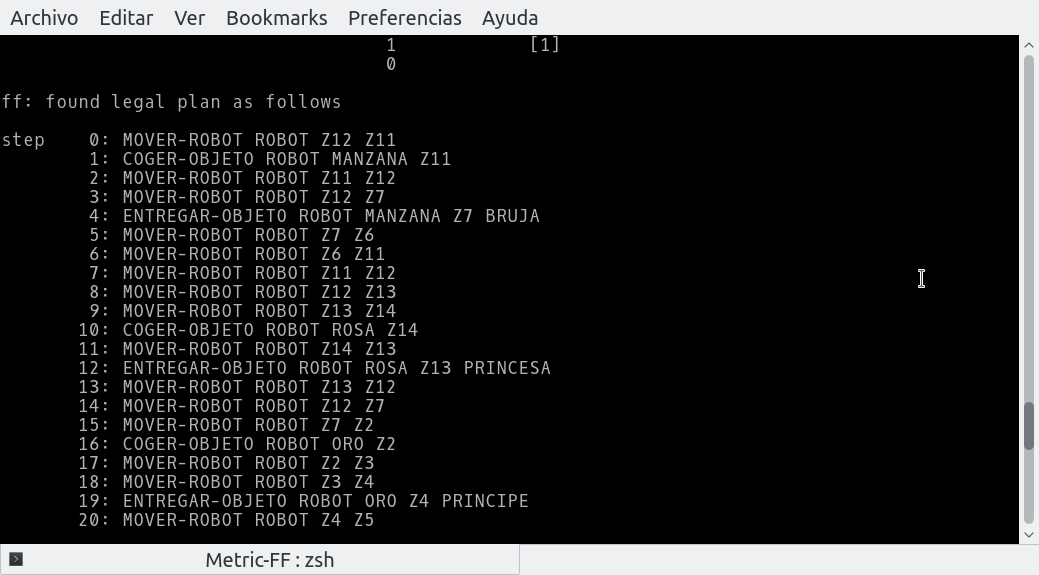
\includegraphics[width=0.8\textwidth]{img1}
	\caption{Primera parte del plan encontrado}
\end{figure}
\begin{figure}[H]
	\centering
	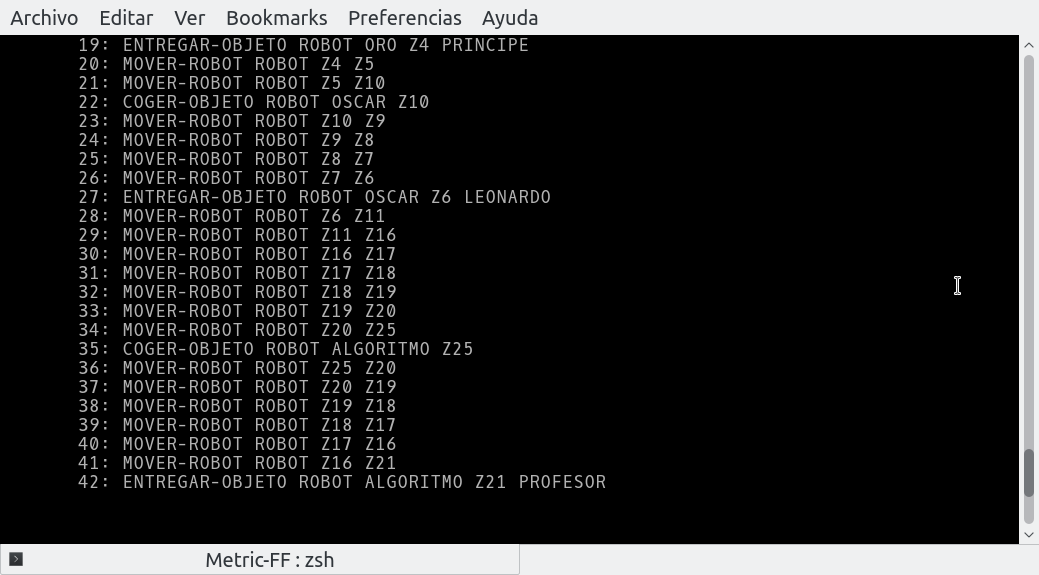
\includegraphics[width=0.8\textwidth]{img2}
	\caption{Primera parte del plan encontrado}
\end{figure}

\section{Ejercicio 2}
\subsection{Apartado a}
Para añadir está característica se ha usado una función coste-fuel para indicar el fuel que se ha gastado, de la siguiente forma:
\begin{verbatim}
(:functions
    (coste-fuel) ;representa el fuel del robot
)
\end{verbatim}
No se ha añadido ningún predicado nuevo, pero con cada movimiento del robot, se consume fuel, por lo que se ha añadido un incremento de fuel como efecto de la acción \textbf{mover-robot}:
\begin{verbatim}
;Acción de movimiento del robot
(:action mover-robot
    :parameters (?r - robot ?z1 - zona ?z2 - zona)
    :precondition (and (not (at ?r ?z2))(at ?r ?z1)(conectada ?z1 ?z2))
    :effect (and (not (at ?r ?z1))(at ?r ?z2)(increase (coste-fuel) 1))
)
\end{verbatim}
\subsection{Apartado b}
El dominio del problema se ha modificado en los siguientes aspectos:
\begin{itemize}
	\item Se ha añadido en :init un nuevo predicado que nos dice que el coste del fuel al comienzo es 0.
	\begin{verbatim}
	(= (coste-fuel) 0)
	\end{verbatim}
	\item Se ha añadido que queremos que el plan minimize el coste de fuel de la siguiente forma:
	\begin{verbatim}
	(:metric minimize (coste-fuel))
	\end{verbatim}
\end{itemize}
El resto es exactamente igual que el apartado d del ejercicio 1.

Podemos observar su correcto funcionamiento en las siguientes imágenes:
\begin{figure}[H]
	\centering
	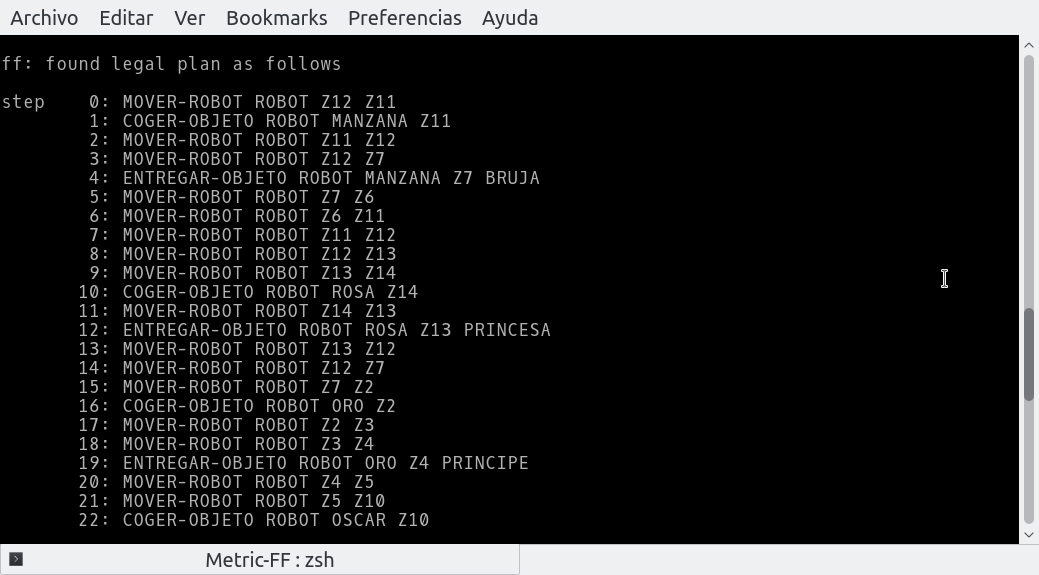
\includegraphics[width=0.8\textwidth]{img3}
	\caption{Primera parte del plan encontrado para el segundo ejercicio}
\end{figure}
\begin{figure}[H]
	\centering
	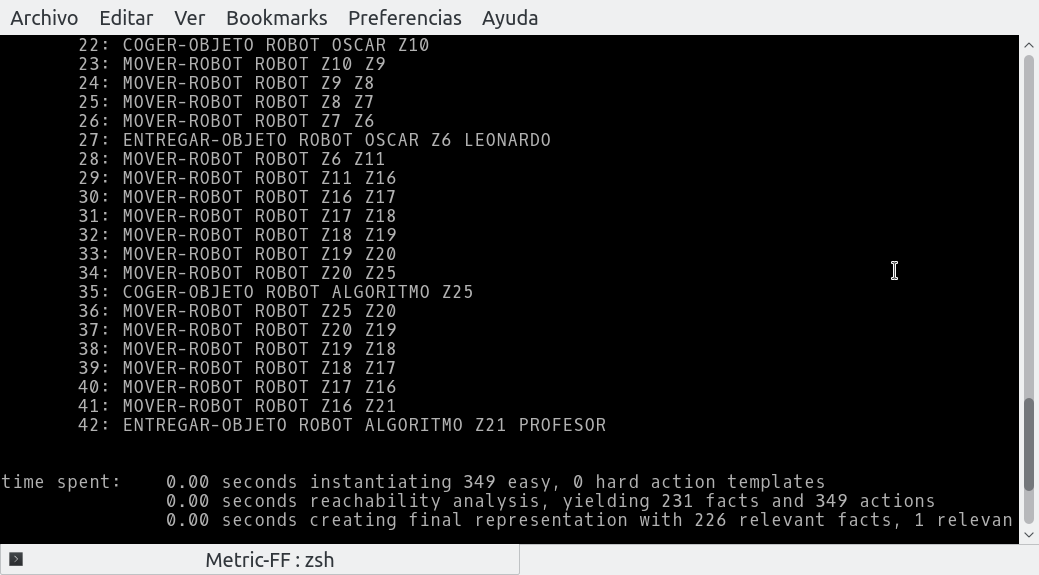
\includegraphics[width=0.8\textwidth]{img4}
	\caption{Segunda parte del plan encontrado para el segundo ejercicio}
\end{figure}
\section{Ejercicio 3}
\subsection{Apartado a}
Para tener en consideración las restricciones se han realizado los siguientes cambios en el dominio anteriormente usado:
\begin{enumerate}
	\item Se ha añadido un nuevo type llamado \textbf{tipo} para determinar el tipo de la zona, y un nuevo type llamado mochila, para trabajar con esta misma.
	\begin{verbatim}
	 (:types robot zona objeto personaje tipo mochila)
	\end{verbatim}
	\item Se ha añadido una nueva función para determinar el coste de una zona según el tipo de la misma.
	\begin{verbatim}
	(coste-zona ?z - tipo) ;coste de una zona
	\end{verbatim}
	\item Se han añadido los siguientes predicados nuevos:
		\subitem \textbf{(mochilavacia)}: indica que la mochila se encuentra vacía.
		\subitem \textbf{(contiene ?x - objeto)}: indica que la mochila contiene un determinado objeto.
		\subitem \textbf{(clase ?x - zona ?y - tipo)}: indica de que tipo es una determinada zona.
		\subitem \textbf{(permite-avanzar ?x - objeto ?y - tipo)}: indica para un determinado tipo de zona que objeto debemos tener para poder avanzar por esa zona.
		\subitem \textbf{(sin-objeto-necesario ?x - tipo)}: indica que un tipo de zona no necesita ningún objeto para poder avanzar por ella.
	\item También se han realizado las siguientes modificaciones en la acción de mover-robot:
		\subitem -Tenga cogido o en la mochila el objeto si quiere pasar por una zona que lo necesite
		\subitem -Se compruebe si se necesita objeto para pasar por el tipo de la zona que quiere.
		\subitem -La diferencia entre el coste de fuel que tiene y el coste de la zona sea mayor o igual a 0.
		\subitem -Ahora se decrementa el fuel según el coste de la zona.	
		\begin{verbatim}
		;Acción de movimiento del robot
		(:action mover-robot
		    :parameters (?r - robot ?z1 - zona ?z2 - zona ?t - tipo ?obj - objeto)
		    :precondition (and (not (at ?r ?z2))(at ?r ?z1)(conectada ?z1 ?z2)
		    (or(cogido ?obj)(contiene ?obj))(or (permite-avanzar ?obj ?t)
		    (sin-objeto-necesario ?t))(>=(-(coste-fuel)(coste-zona ?t))0))
		    :effect (and (not (at ?r ?z1))(at ?r ?z2)
		    (decrease (coste-fuel)(coste-zona ?t)))
		)
		\end{verbatim}
\end{enumerate}
\subsection{Apartado b}
Para ello se han añadido las siguientes acciones:
\begin{enumerate}
	\item \textbf{meter-mochila}
	\begin{verbatim}
	;Guardar un objeto en la mochila
	(:action meter-mochila
	    :parameters(?r - robot ?obj - objeto)
	    :precondition(and (cogido ?obj)(mochilavacia))
	    :effect(and (not (cogido ?obj))(not (mochilavacia))(manovacia)(contiene ?obj))
	)
	\end{verbatim}
	Para poder meter un objeto en la mochila, la mochila debe estar vacía, y debmos tener el objeto cogido.
	\item \textbf{sacar-mochila}
	\begin{verbatim}
	;Sacar un objeto de la mochila
	(:action sacar-mochila
	     :parameters(?r - robot ?obj - objeto)
	     :precondition(and (contiene ?obj)(manovacia))
	     :effect(and (not (contiene ?obj))(not (manovacia))(mochilavacia)(cogido ?obj))
	)
	\end{verbatim}
	Para poder sacar el objeto de la mochila debe tenerlo, por supuesto, y además debe tener la mano vacía.
\end{enumerate}
\subsection{Apartado c}
Las modificaciones que se han realizado al archivo de problema anterior son las siguientes:
\begin{enumerate}
	\item Se han añadido los objetos zapatilla y bikini, además de los tipos de zonas.
	\begin{verbatim}
	OSCAR MANZANA ROSA ALGORITMO ORO ZAPATILLA BIKINI - objeto
	BOSQUE AGUA PRECIPICIO ARENA PIEDRA - tipo
	\end{verbatim}
	\item Se han añadido los siguientes predicados nuevos y modificado el de coste-fuel y se ha puesto a valor 100:
	\begin{verbatim}
	(MOCHILAVACIA)
	(CLASE Z1 PRECIPICIO)
	(CLASE Z2 PIEDRA)
	(CLASE Z3 PIEDRA)
	(CLASE Z4 PIEDRA)
	(CLASE Z5 PIEDRA)
	(CLASE Z6 PIEDRA)
	(CLASE Z7 BOSQUE)
	(CLASE Z8 BOSQUE)
	(CLASE Z9 BOSQUE)
	(CLASE Z10 AGUA)
	(CLASE Z11 AGUA)
	(CLASE Z12 AGUA)
	(CLASE Z13 AGUA)
	(CLASE Z14 AGUA)
	(CLASE Z15 AGUA)
	(CLASE Z16 ARENA)
	(CLASE Z17 ARENA)
	(CLASE Z18 ARENA)
	(CLASE Z19 ARENA)
	(CLASE Z20 ARENA)
	(CLASE Z21 BOSQUE)
	(CLASE Z22 BOSQUE)
	(CLASE Z23 PRECIPICIO)
	(CLASE Z24 BOSQUE)
	(CLASE Z25 BOSQUE)
	(PERMITE-AVANZAR BIKINI AGUA)
	(PERMITE-AVANZAR ZAPATILLA BOSQUE)
	(SIN-OBJETO-NECESARIO PIEDRA)
	(SIN-OBJETO-NECESARIO ARENA)
	(AT1 BIKINI Z12)
	(AT1 ZAPATILLA Z21)
	(= (coste-zona PRECIPICIO) 10000)
	(= (coste-zona AGUA) 1)
	(= (coste-zona BOSQUE) 2)
	(= (coste-zona ARENA) 1)
	(= (coste-zona PIEDRA) 3)
	(= (coste-fuel) 100)
	\end{verbatim}
\end{enumerate}
En las siguientes imágenes podemos observar como encuentra un plan:
\begin{figure}[H]
	\centering
	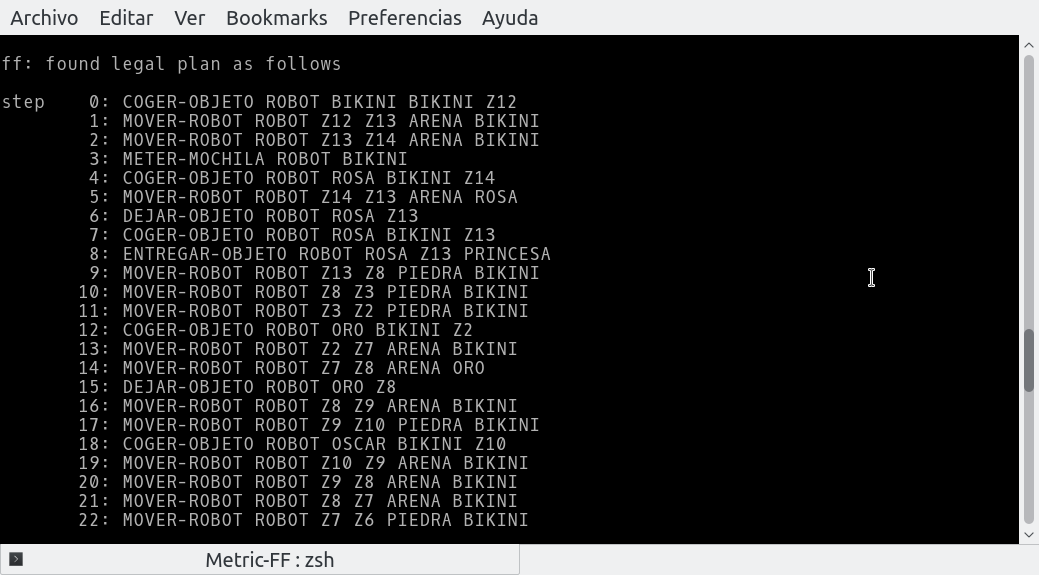
\includegraphics[width=0.8\textwidth]{img5}
	\caption{Primera parte del plan encontrado para el tercer ejercicio}
\end{figure}
\begin{figure}[H]
	\centering
	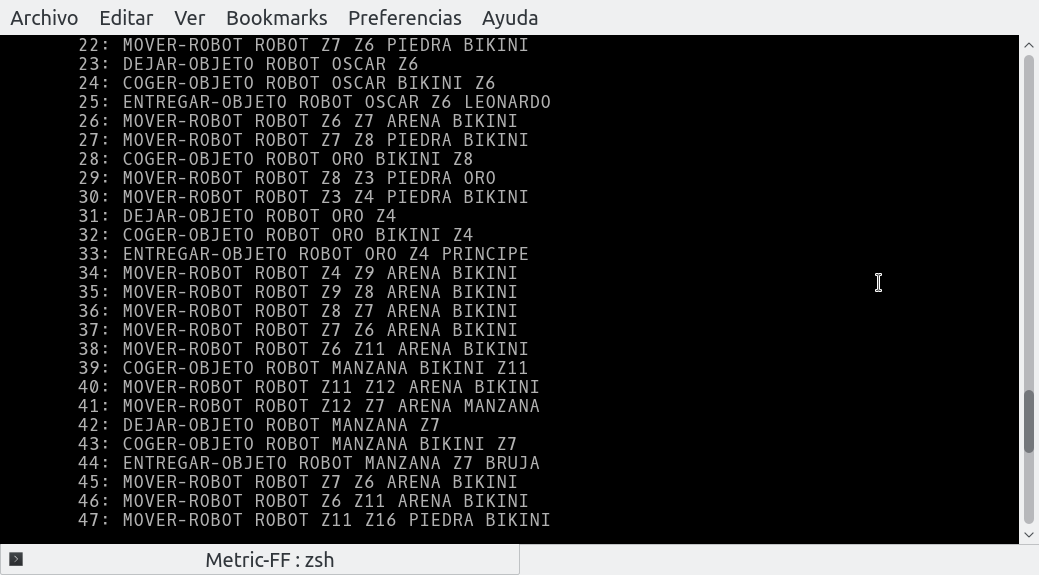
\includegraphics[width=0.8\textwidth]{img6}
	\caption{Segunda parte del plan encontrado para el tercer ejercicio}
\end{figure}
\begin{figure}[H]
	\centering
	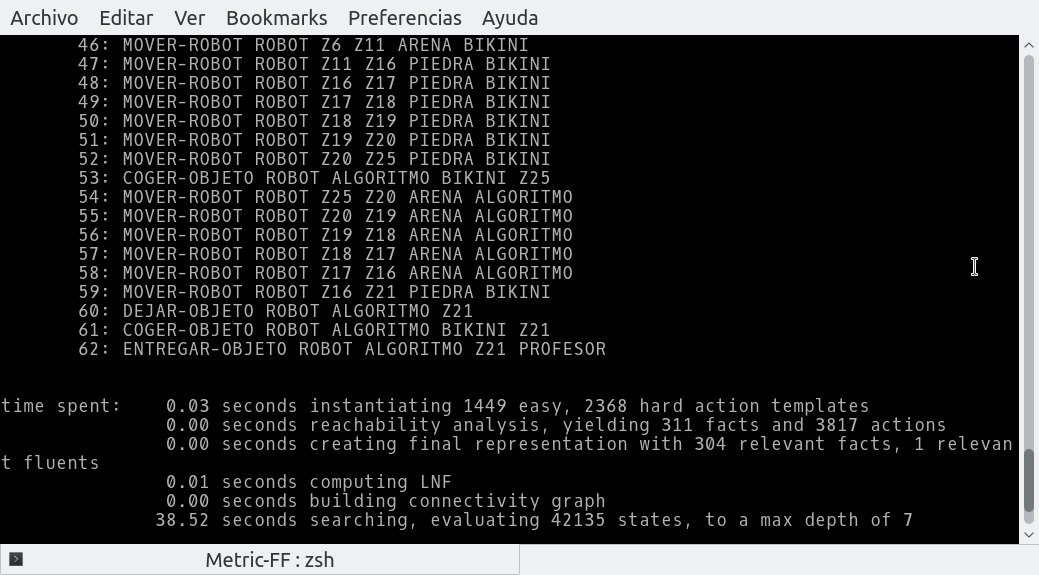
\includegraphics[width=0.8\textwidth]{img7}
	\caption{Tercera parte del plan encontrado para el tercer ejercicio}
\end{figure}
\section{Ejercicio 4}
\subsection{Apartado a}
Se han añadido las siguientes funciones para poder contar los puntos de cada personaje y los puntos objetivo que queremos alcanzar:
\begin{verbatim}
(suma-puntos ?x - objeto ?y - personaje) ;Suma puntos de los personajes
(puntos)
\end{verbatim}
Con \textit{suma-puntos} le indicamos que puntos le corresponden a la pareja de un objeto y un personaje determinado.\\
Con \textit{puntos} determinamos la cantidad de puntos que queremos alcanzar como goal del problema.\\
Además la acción \textit{entregar-objeto} se ha modificado para que incremente el número de puntos según el objeto que le damos al personaje, como podemos obervar a continuación. 
\begin{verbatim}
;Entregar un objeto a un personaje
(:action entregar-objeto
     :parameters(?r - robot ?obj - objeto ?z - zona ?p - personaje)
     :precondition (and (not (tiene ?obj ?p))(at ?r ?z)(at1 ?obj ?z)(at2 ?p ?z)
     (cogido ?obj))
     :effect (and (not (cogido ?obj))(tiene ?obj ?p)(manovacia)
     (increase (puntos) (suma-puntos ?obj ?p)))
)
\end{verbatim}
\subsection{Apartado b}
Del problema del ejercicio 3 se han modificado los siguientes puntos para adaptarlo a estas nuevas condiciones:
\begin{enumerate}
	\item Se han añadido todos los puntos correspondientes según el objeto y el personaje, según se nos indica en el enunciado del ejercicio.
	\item Se inicializa el valor de puntos que se tiene al comienzo a 0.
	\item Se cambia el goal por el número de puntos que deseamos alcanzar.
\end{enumerate}
Se pueden observar los cambios a continuación:
\begin{verbatim}
(= (suma-puntos OSCAR LEONARDO) 10)
(= (suma-puntos OSCAR PRINCESA) 5)
(= (suma-puntos OSCAR BRUJA) 4)
(= (suma-puntos OSCAR PROFESOR) 3)
(= (suma-puntos OSCAR PRINCIPE) 1)
(= (suma-puntos ROSA LEONARDO) 1)
(= (suma-puntos ROSA PRINCESA) 10)
(= (suma-puntos ROSA BRUJA) 5)
(= (suma-puntos ROSA PROFESOR) 4)
(= (suma-puntos ROSA PRINCIPE) 3)
(= (suma-puntos MANZANA LEONARDO) 3)
(= (suma-puntos MANZANA PRINCESA) 1)
(= (suma-puntos MANZANA BRUJA) 10)
(= (suma-puntos MANZANA PROFESOR) 5)
(= (suma-puntos MANZANA PRINCIPE) 4)
(= (suma-puntos ALGORITMO LEONARDO) 4)
(= (suma-puntos ALGORITMO PRINCESA) 3)
(= (suma-puntos ALGORITMO BRUJA) 1)
(= (suma-puntos ALGORITMO PROFESOR) 10)
(= (suma-puntos ALGORITMO PRINCIPE) 5)
(= (suma-puntos ORO LEONARDO) 5)
(= (suma-puntos ORO PRINCESA) 4)
(= (suma-puntos ORO BRUJA) 3)
(= (suma-puntos ORO PROFESOR) 1)
(= (suma-puntos ORO PRINCIPE) 10)
(= (puntos) 0)

)

(:goal (= (puntos) 50))
)
\end{verbatim}
En las siguientes imágenes podemos observar como encuentra un plan:
\begin{figure}[H]
	\centering
	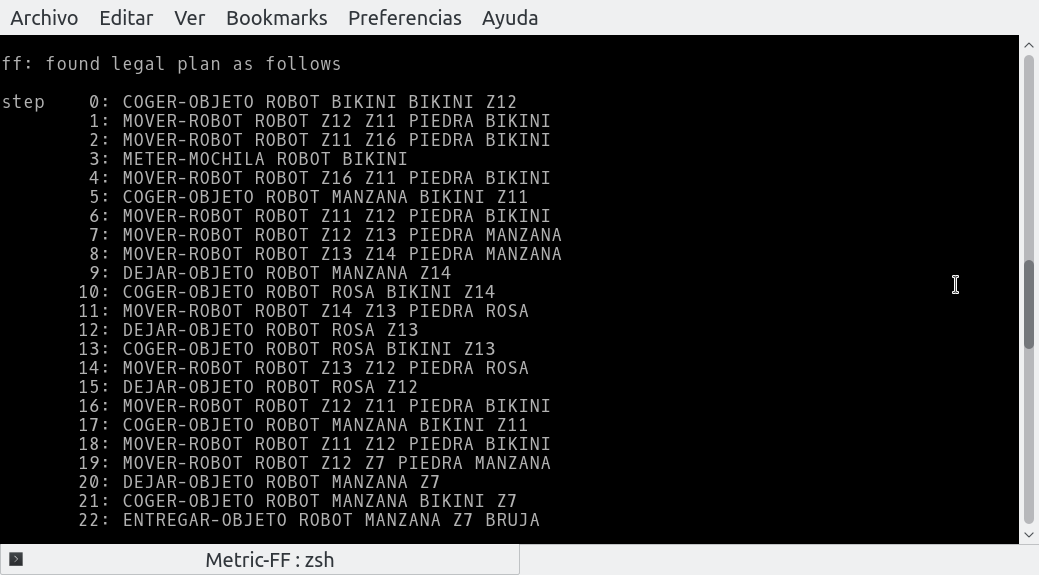
\includegraphics[width=0.8\textwidth]{img8}
	\caption{Primera parte del plan encontrado para el cuerto ejercicio}
\end{figure}
\begin{figure}[H]
	\centering
	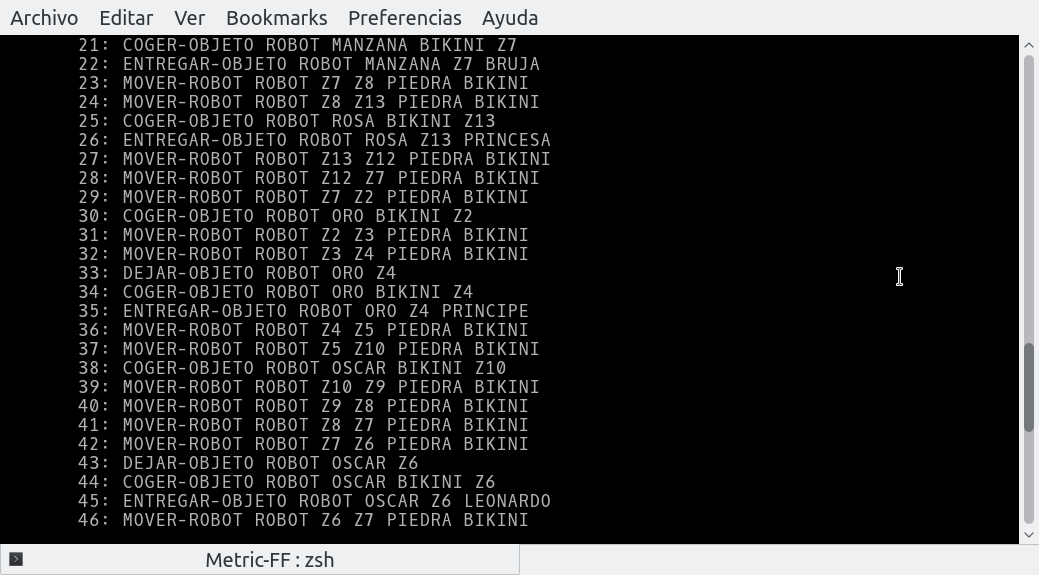
\includegraphics[width=0.8\textwidth]{img9}
	\caption{Segunda parte del plan encontrado para el cuarto ejercicio}
\end{figure}
\begin{figure}[H]
	\centering
	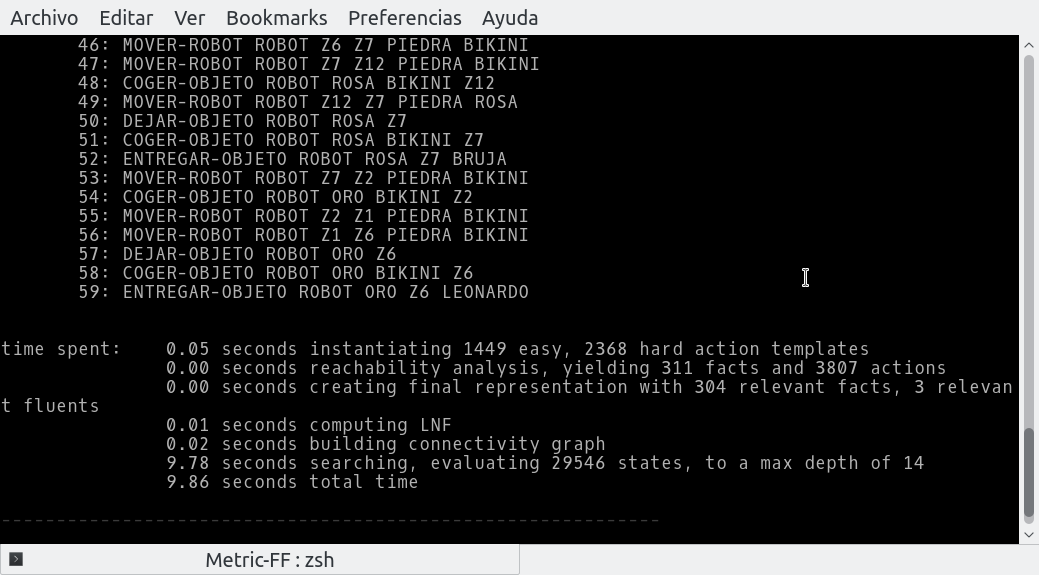
\includegraphics[width=0.8\textwidth]{img10}
	\caption{Tercera parte del plan encontrado para el cuarto ejercicio}
\end{figure}
\section{Ejercicio 5}
\subsection{Apartado a}
Para trabajar con la capacidad de la mochila se han añadido dos nuevas funciones:
\begin{enumerate}
	\item \textbf{(capacidad)}: que indica la capacidad de la mochila.
	\item \textbf{(objetos-mochila)}: cantidad de objetos que llevo actualmente en la mochila.
\end{enumerate}
En la acción de mover no se ha modificado, ya que consideraba si había algo en la mochila, y esto es indiferente al número de objetos que se encuentren en ella. En cambio, las acciones de cargar y sacar de la mochila se han modificado de la siguiente forma:
\begin{verbatim}
;Guardar un objeto en la mochila
(:action meter-mochila
    :parameters(?r - robot ?obj - objeto)
    :precondition(and (cogido ?obj)(>(- (capacidad)(objetos-mochila))0))
    :effect(and (not (cogido ?obj))(manovacia)(contiene ?obj)
    (increase (objetos-mochila)1))
)
;Sacar un objeto de la mochila
(:action sacar-mochila
    :parameters(?r - robot ?obj - objeto)
    :precondition(and (contiene ?obj)(manovacia))
    :effect(and (not (contiene ?obj))(not (manovacia))(cogido ?obj)
    (decrease (objetos-mochila)1))
)
\end{verbatim}
\subsection{Apartado b}
Se ha extendido el fichero de problema anterior añadiendo la capacidad de la mochila que queramos, y indicando que comenzamos con 0 objetos en la mochila:
\begin{verbatim}
= (capacidad) 3)
(= (objetos-mochila) 0)
\end{verbatim}
En las siguientes imágenes podemos observar como encuentra un plan:
\begin{figure}[H]
	\centering
	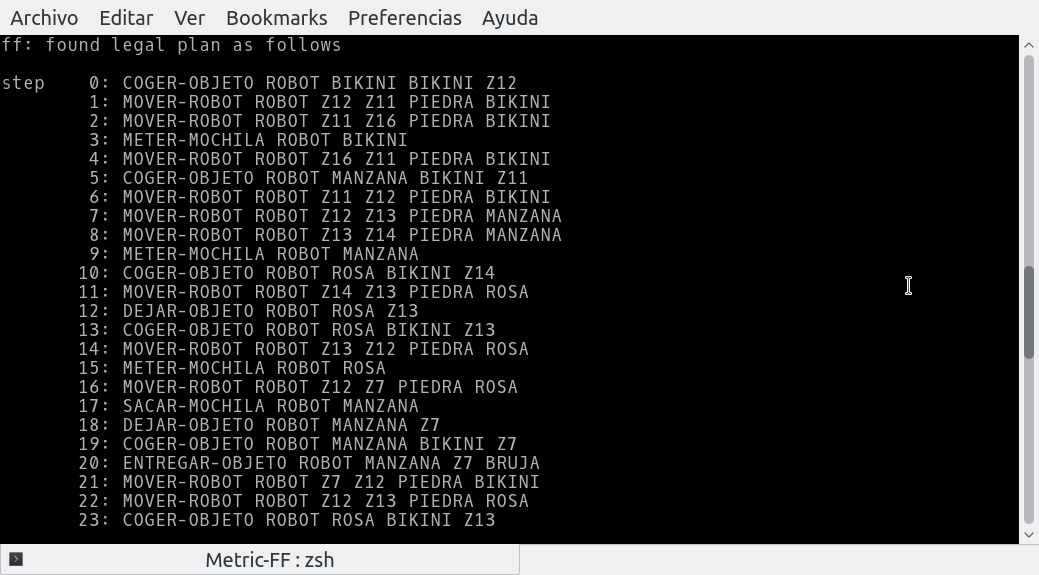
\includegraphics[width=0.8\textwidth]{img11}
	\caption{Primera parte del plan encontrado para el quinto ejercicio}
\end{figure}
\begin{figure}[H]
	\centering
	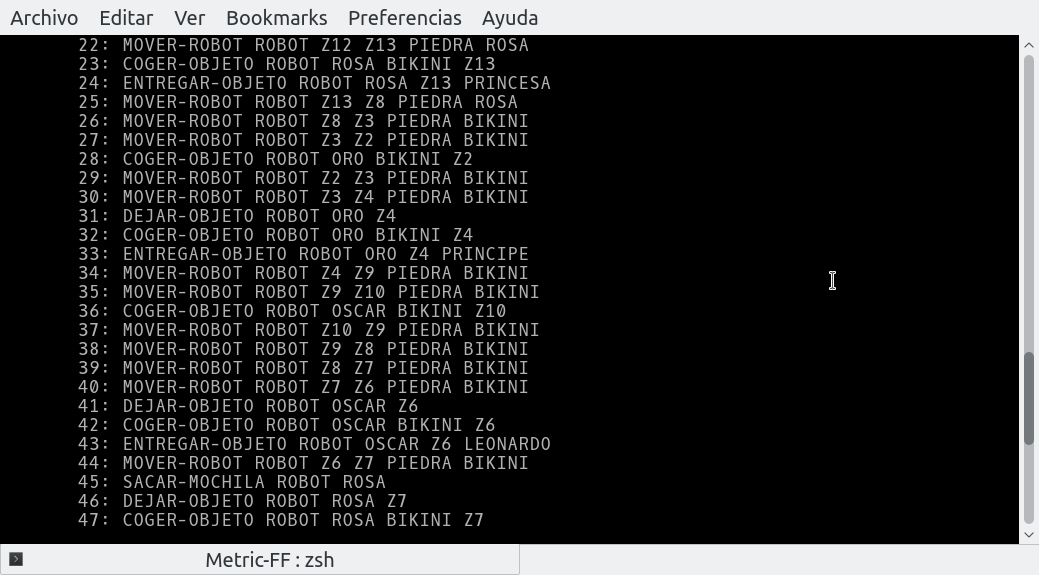
\includegraphics[width=0.8\textwidth]{img12}
	\caption{Segunda parte del plan encontrado para el quinto ejercicio}
\end{figure}
\begin{figure}[H]
	\centering
	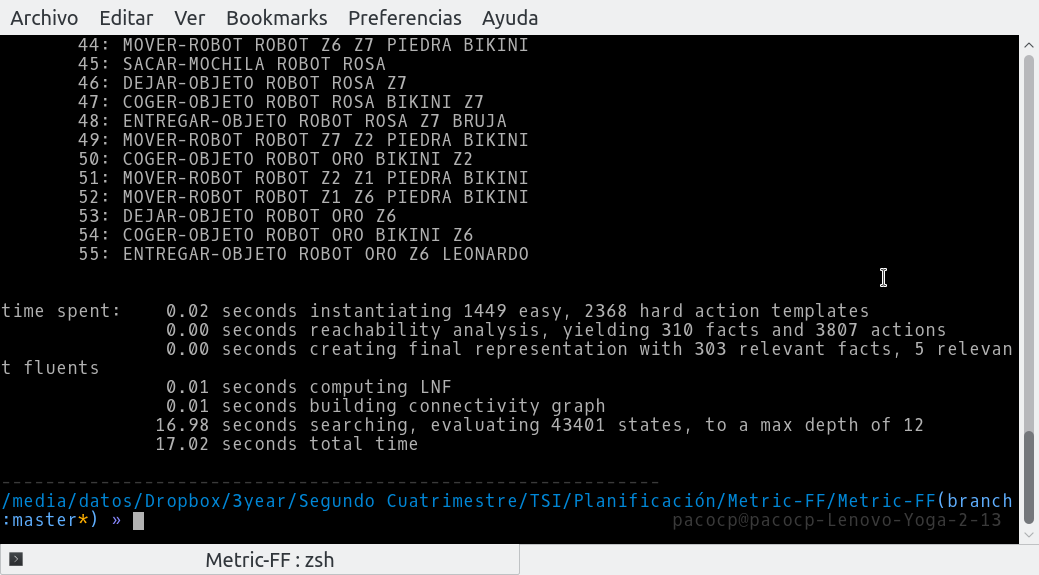
\includegraphics[width=0.8\textwidth]{img13}
	\caption{Tercera parte del plan encontrado para el quinto ejercicio}
\end{figure}
Se puede observar por tanto que encuentra un plan con menos pasos, ya que en este caso son 55 pasos, y con el problema del ejercicio 4 eran 59 pasos.
\end{document}